\documentclass[a4paper]{article}


\usepackage[T1]{fontenc}
\usepackage[utf8]{inputenc}
\usepackage{mathptmx}

%\usepackage{ngerman}	% Sprachanpassung Deutsch

\usepackage{graphicx}
\usepackage{geometry}
\geometry{a4paper, top=15mm}

\usepackage{subcaption}
\usepackage[shortlabels]{enumitem}
\usepackage{amssymb}
\usepackage{amsthm}
\usepackage{mathtools}
\usepackage{braket}
\usepackage{bbm}
\usepackage{graphicx}
\usepackage{float}
\usepackage{yhmath}
\usepackage{tikz}
\usetikzlibrary{patterns,decorations.pathmorphing,positioning}
\usetikzlibrary{calc,decorations.markings}

\usepackage[backend=biber, sorting=none]{biblatex}
\addbibresource{uni.bib}

\usepackage[framemethod=TikZ]{mdframed}

\tikzstyle{titlered} =
    [draw=black, thick, fill=white,%
        text=black, rectangle,
        right, minimum height=.7cm]


\usepackage[colorlinks=true,naturalnames=true,plainpages=false,pdfpagelabels=true]{hyperref}
\usepackage[parfill]{parskip}
\usepackage{lipsum}


\usepackage{tcolorbox}
\tcbuselibrary{skins,breakable}

\pagestyle{myheadings}

\markright{Popovic\hfill 1st Exercise \hfill}


\title{University of Vienna\\ Faculty of Mathematics\\
\vspace{1cm}TENSOR METHODS FOR DATA SCIENCE AND SCIENTIFIC COMPUTING \\ 1st
Exercise
}
\author{Milutin Popovic}
\date{24. October, 2021}

\begin{document}
\maketitle
\tableofcontents

\section{Introduction}
In the following we consider two functions $f$ and $g$ defined pointwise on
$[-1, 1]^2$ as
\begin{align}
    f(x, y) &:= \frac{1}{1+x^2+y^2} \;\;\; \text{and}\\
    g(x, y) &:= \sqrt{x^2+y^2}\cdot\left(1+\frac{1}{2}cos(15x + 22x)\right),
\end{align}
for $x, y \in [-1, 1]$, with a grid of points $t$ of size $n=901$
\begin{align}
    t_i = 2\frac{i-1}{n-1}-1 \;\;\;\;\;\; i=1,\dots,n.
\end{align}
On this $n\times n$ grid we define two matrices $A$ and $B$ as the following
\begin{align}
    (A)_{ij} &= a_{ij} := f(t_i, t_j)\;\;\; \text{and}\\
    (B)_{ij} &= b_{ij} := g(t_i, t_j),
\end{align}
for all $i, j \in \{1,\dots, n\}$. Throughout we denote $r$ as the rank of the
approximate factorization of $A$ or $B$, which actually only makes sense for
$r \leq rank(A)$ or $r \leq rank(B)$ accordingly. Since the matrices $A$ and
$B$ have the following ranks
\begin{align}
    rank(A) = 8 \;\;\;\;\;\; rank(B) = 57,
\end{align}
only low rank approximations are valid and any rank approximation above the
matrix rank is not valid, e.g. $r=80$ approximation does not make any sense.

\section{Matrix approximation by SVD}
In this section we go through the error analysis in Forbenius and max norms
of the truncated SVD on the matrices $A$ and $B$. Considering a $n \times n$
(real or complex matrix) $M$ them the truncated SVD of rank $r$ will give
an approximation of $M$, $\tilde{M}$
\begin{align}
    \tilde{M} = U \Sigma V^*,
\end{align}
where $U \in \mathbb{F}^{n \times r}$ ($\mathbb{F} = \mathbb{R}
\;\text{or}\;\; \mathbb{C}$), $\Sigma \in \mathbb{F}^{r \times r}$
with $r$ largest singular values are the diagonal (else zero) and $V^{r
\times n}$. The computational errors of the TSVD approximation of  $A$ and
$B$ are shown in figure \ref{fig:svd-err} below.
\begin{figure}[H]
    \centering
    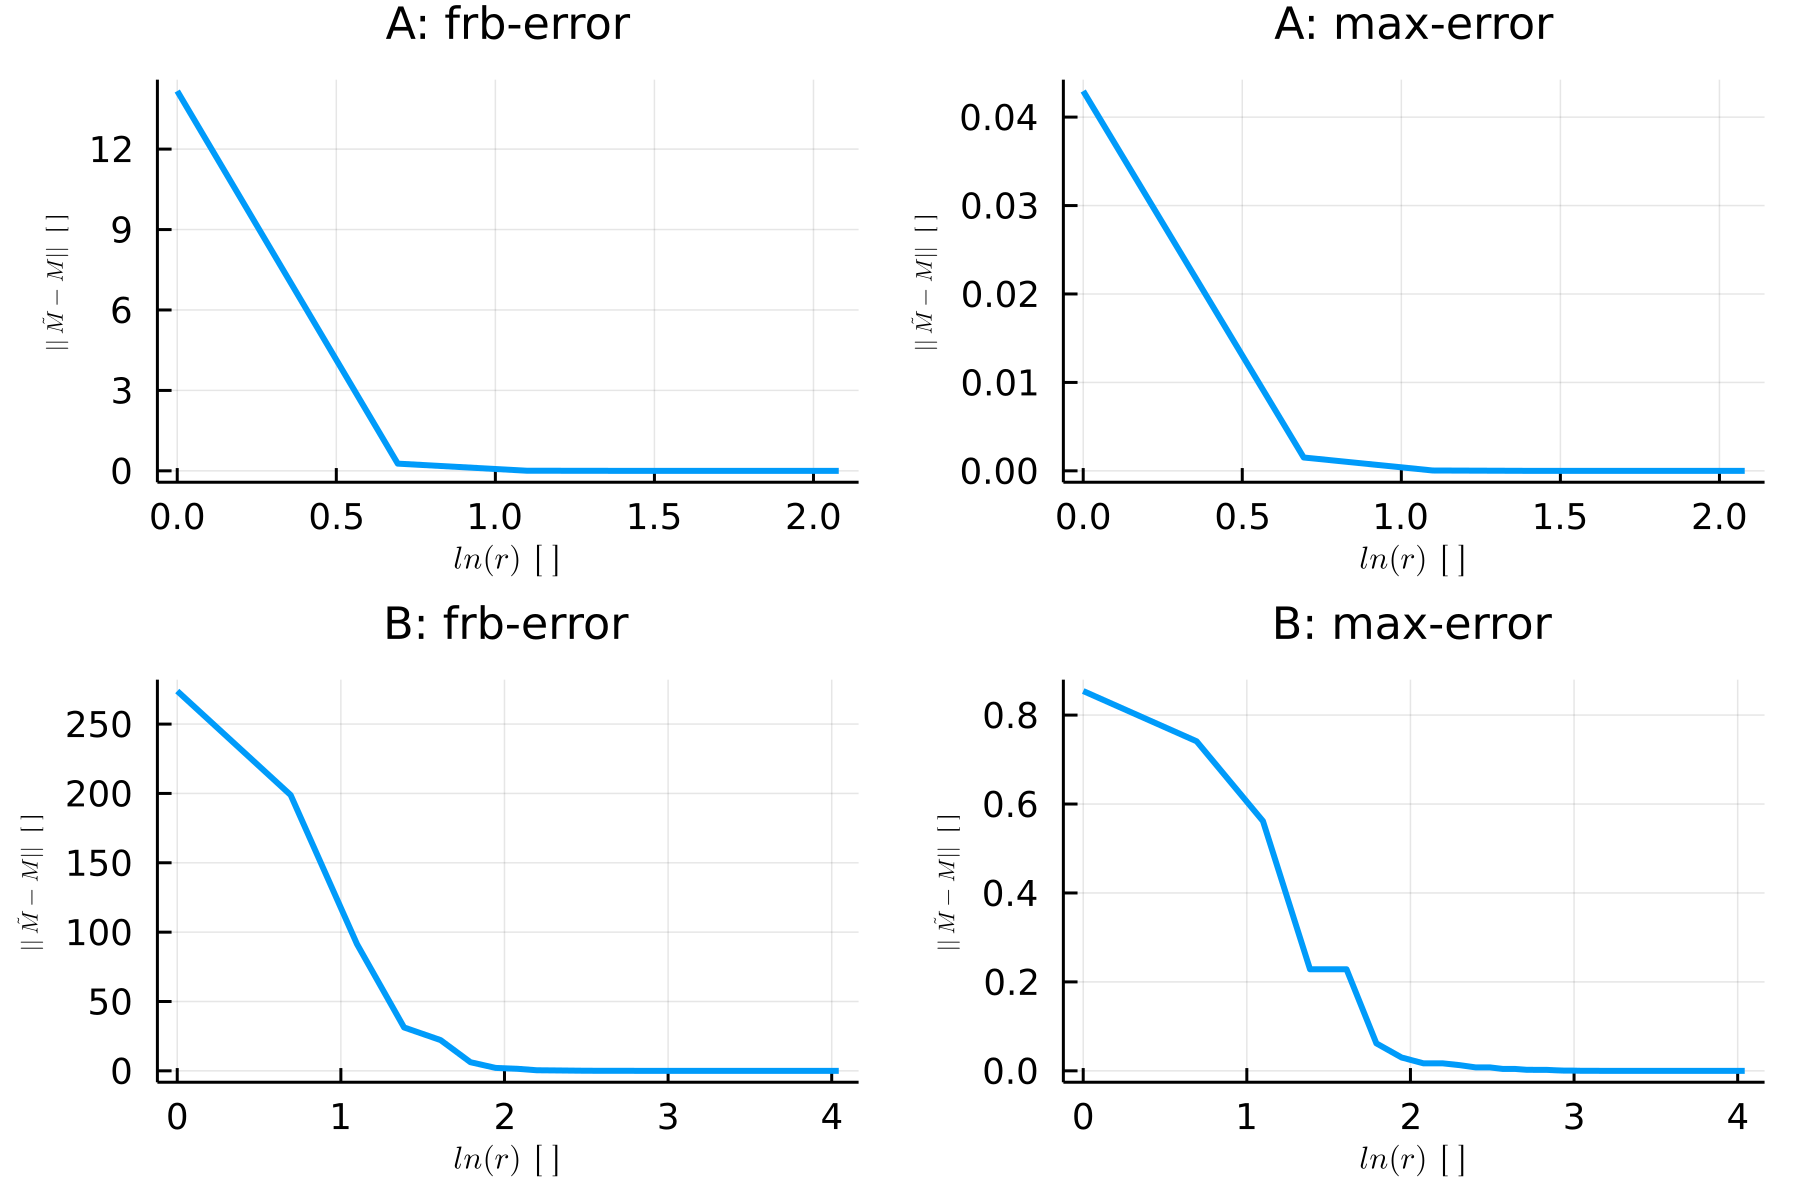
\includegraphics[width=0.8\textwidth]{plots/svd-err.png}
    \caption{\label{fig:svd-err}Error of rank $r$ truncated SVD approximation
    of matrices $A$ and $B$ on a logarithmic scale}
\end{figure}
The error convergance can be explained by applying the Eckart-Young-Mirsky
theorem for functions f, g and their singular value decomposition of rank r explicitly.
In this sense both norms would be equivalent. Since we for a $p =
\{0,\cdots,r\}$ by the lecture script we have
\begin{align}
    A_p = \sum_{k=1}^p \sigma_k u_k v^*_k.
\end{align}
Thus for $r \rightarrow rank(A)$ the sum would converge to the original
matrix $A$ making the difference
\begin{align}
    ||A_p - A||_{F \;\text{or} 2}
\end{align}
minimal, converging to zero.

\section{Matrix approximation by LU without pivoting}
In this section we look at the errors formed by the LU approximation of the
leading principal submatrix without pivoting, when considering rank $r$ cross approximation
of the given matrix. Again we atone, that this procedure does not make sense
for a submatrix of a size above the rank of the original matrix, since for
the approximation the inverse of the submatrix is needed. Also on of the
criteria is that the leading principal submatrix is a matrix with maximal
volume and maximal rank. Obtaining the maximum volume submatrix is very
difficult\cite{survey}, thus we will use an algorithm called ``Maxvol''
\cite{maxvol} to obtain a quasioptimal maximum volume submatrix. In this
let us say we are considering appropriate matrix $M$ to approximate, to
compute the quasioptimal submatrix we first need to select random $r$ columns
of $M$, then the algorithm ``Maxvol'' will do the rest of the work. Further out
we apply the LU decomposition on the leading principal submatrix without
pivoting and construct an approximation of $M$ by the cross approximation (as
in the lecture notes). The computational errors of the LU-cross approximation
without pivoting of $A$ and $B$ are shown in figure \ref{fig:lu-np-err}
below.
\begin{figure}[H]
    \centering
    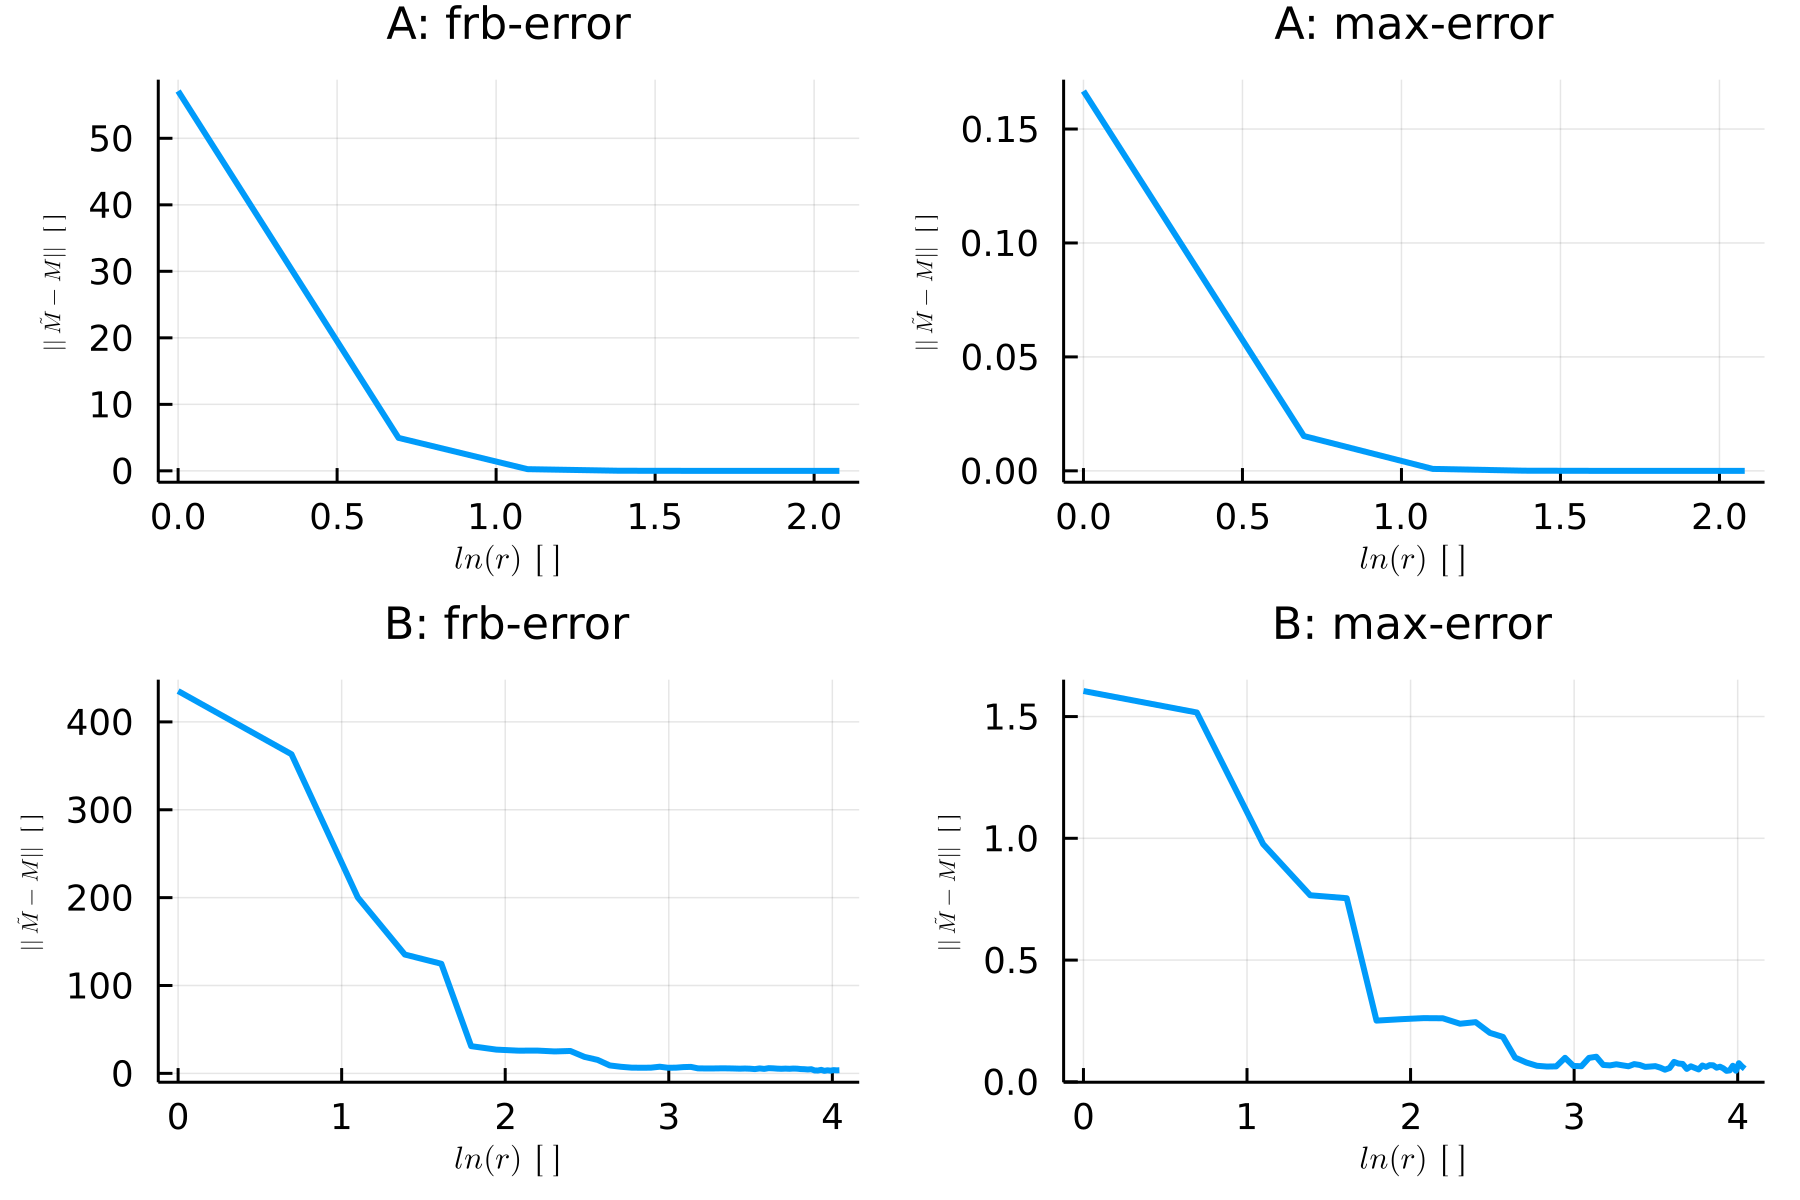
\includegraphics[width=0.8\textwidth]{plots/lu-np-err.png}
    \caption{\label{fig:svd-err}Error of rank $r$ LU-cross approximation
    of matrices $A$ and $B$ on a logarithmic scale without pivoting}
\end{figure}

\section{Matrix approximation by LU with pivoting}
Here we follow the same procedure, where we cross approximate the matrix.
Only that now we consider a pivoted LU decomposition of the leading principal
submatrix.The computational errors of the LU-cross approximation with
pivoting of $A$ and $B$ are shown in figure \ref{fig:lu-np-err} below.
\begin{figure}[H]
    \centering
    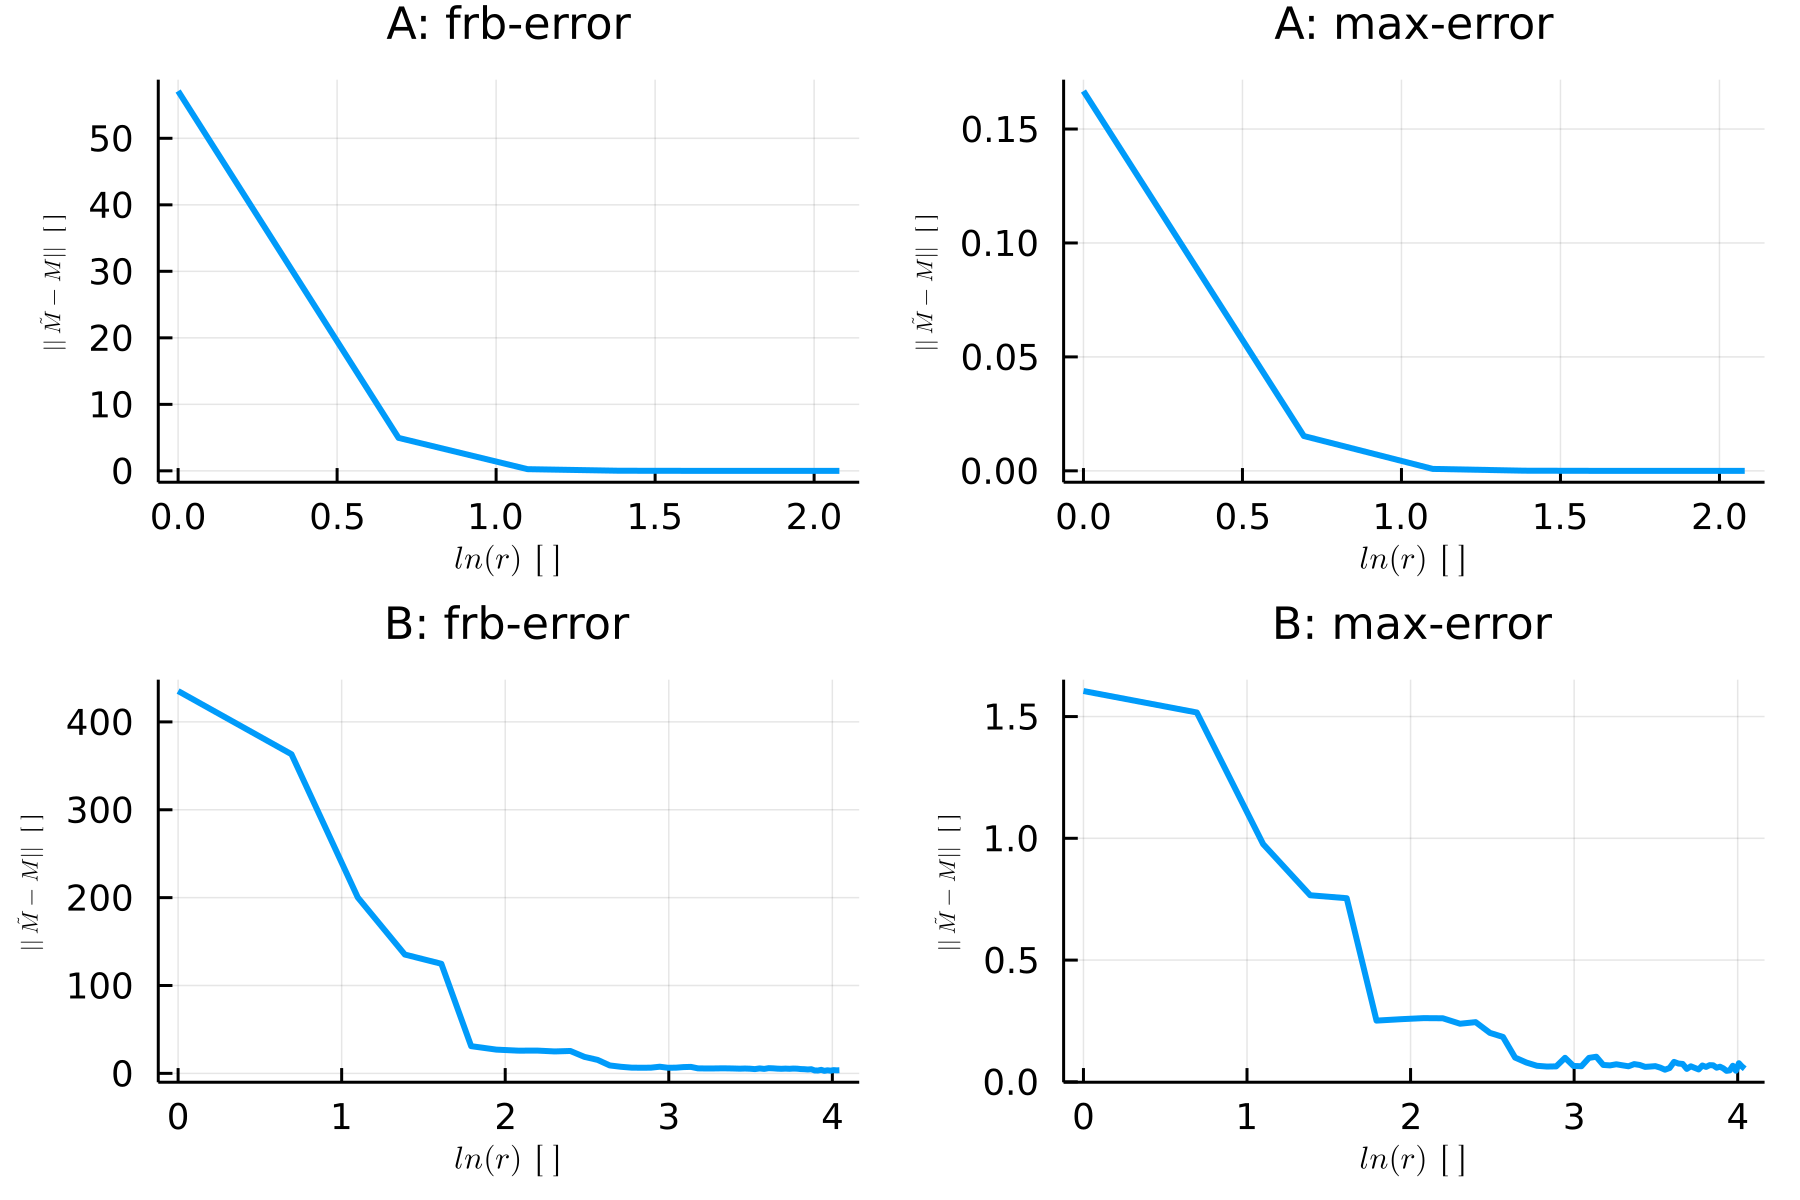
\includegraphics[width=0.8\textwidth]{plots/lu-p-err.png}
    \caption{\label{fig:svd-err}Error of rank $r$ LU-cross approximation
    of matrices $A$ and $B$ on a logarithmic scale with pivoting}
\end{figure}
The convergence observed is that the bigger $r$, the less the error is.
By \cite{error-cross}, for a matrix $A$ and its according leading principal submatrix
$A_11$, of a rank exceeding $r$ we have
\begin{align}
    ||\hat{A}- A||_{F/2} \leq(r+1)^2 \min_{rank(B) \leq r} ||A - B||_{F/2}.
\end{align}
Every increasing of $r$ in the LU-cross approximation we are ``nearer'' the
original matrix $A$.
\section{Understanding the basis rows and columns}
Here we show contour and surface plots of $f$ and $g$ on $[-1, 1]^2$ and
additionally color red the axis-parallel lines selected by the pivoted LU
algorithm above used for the cross approximation at $r = 1, 2, 3, 4, 5, 10,
15, 20, 30, 40$. Where for the matrix $A$ only lines for up to $rank(A) = 8$
are dawn in.
\begin{figure}[H]
    \centering
    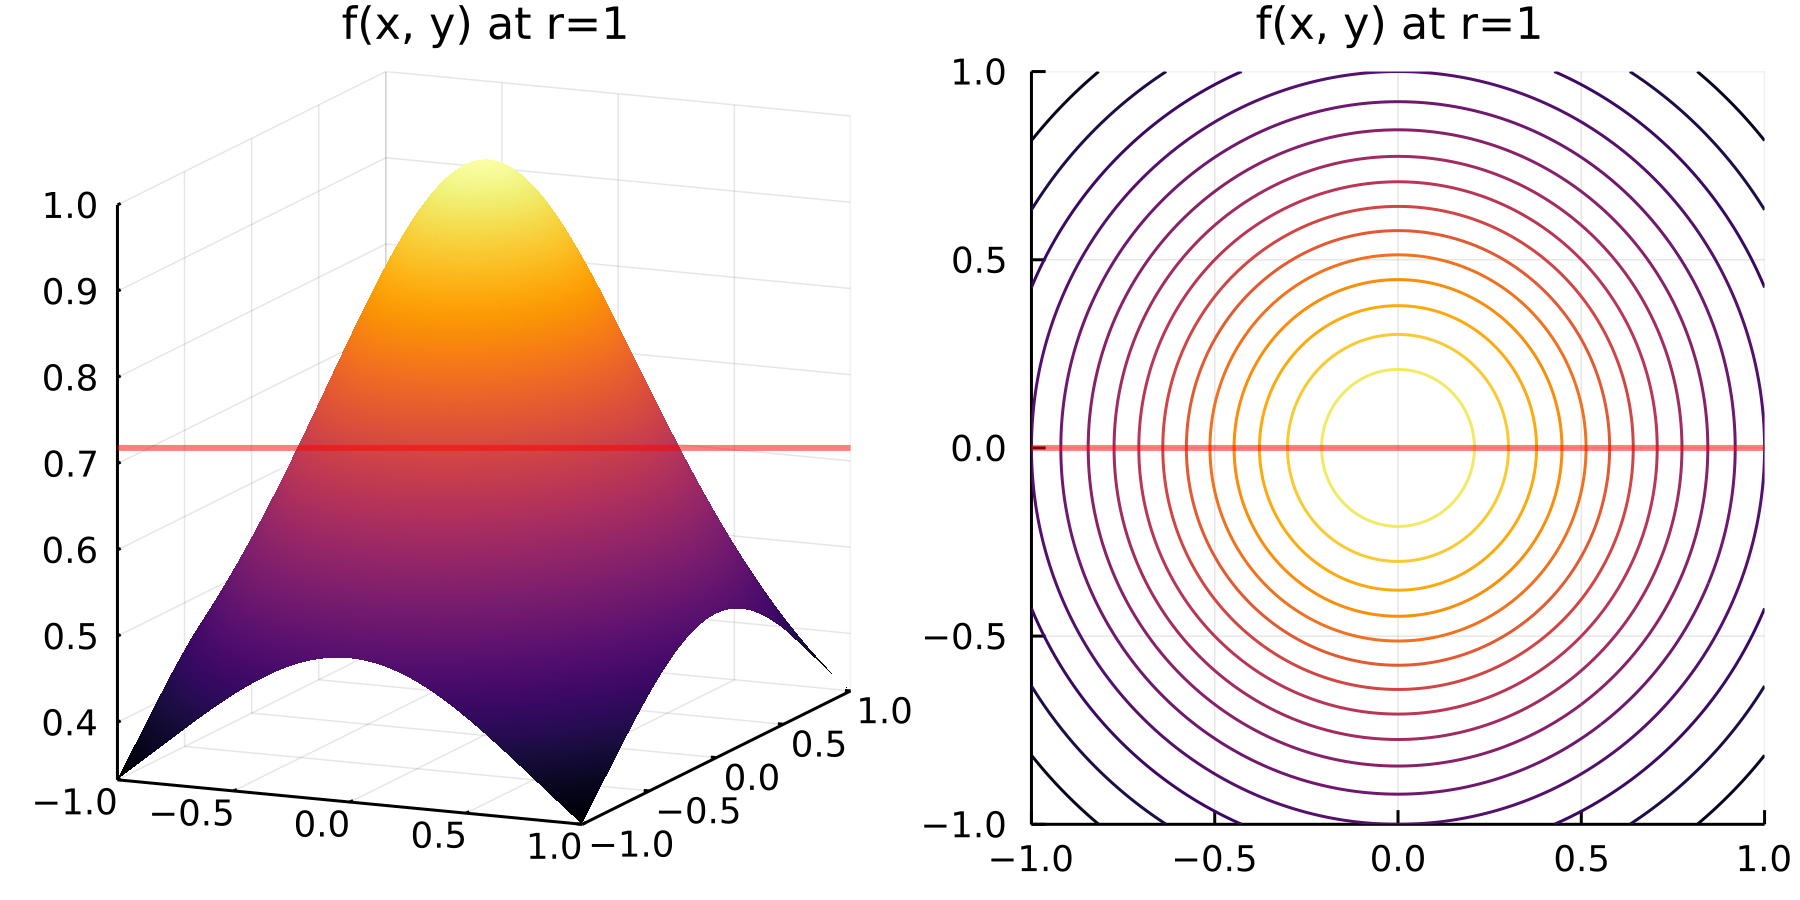
\includegraphics[width=.33\textwidth]{plots/rc-a-1.png}\hfill
    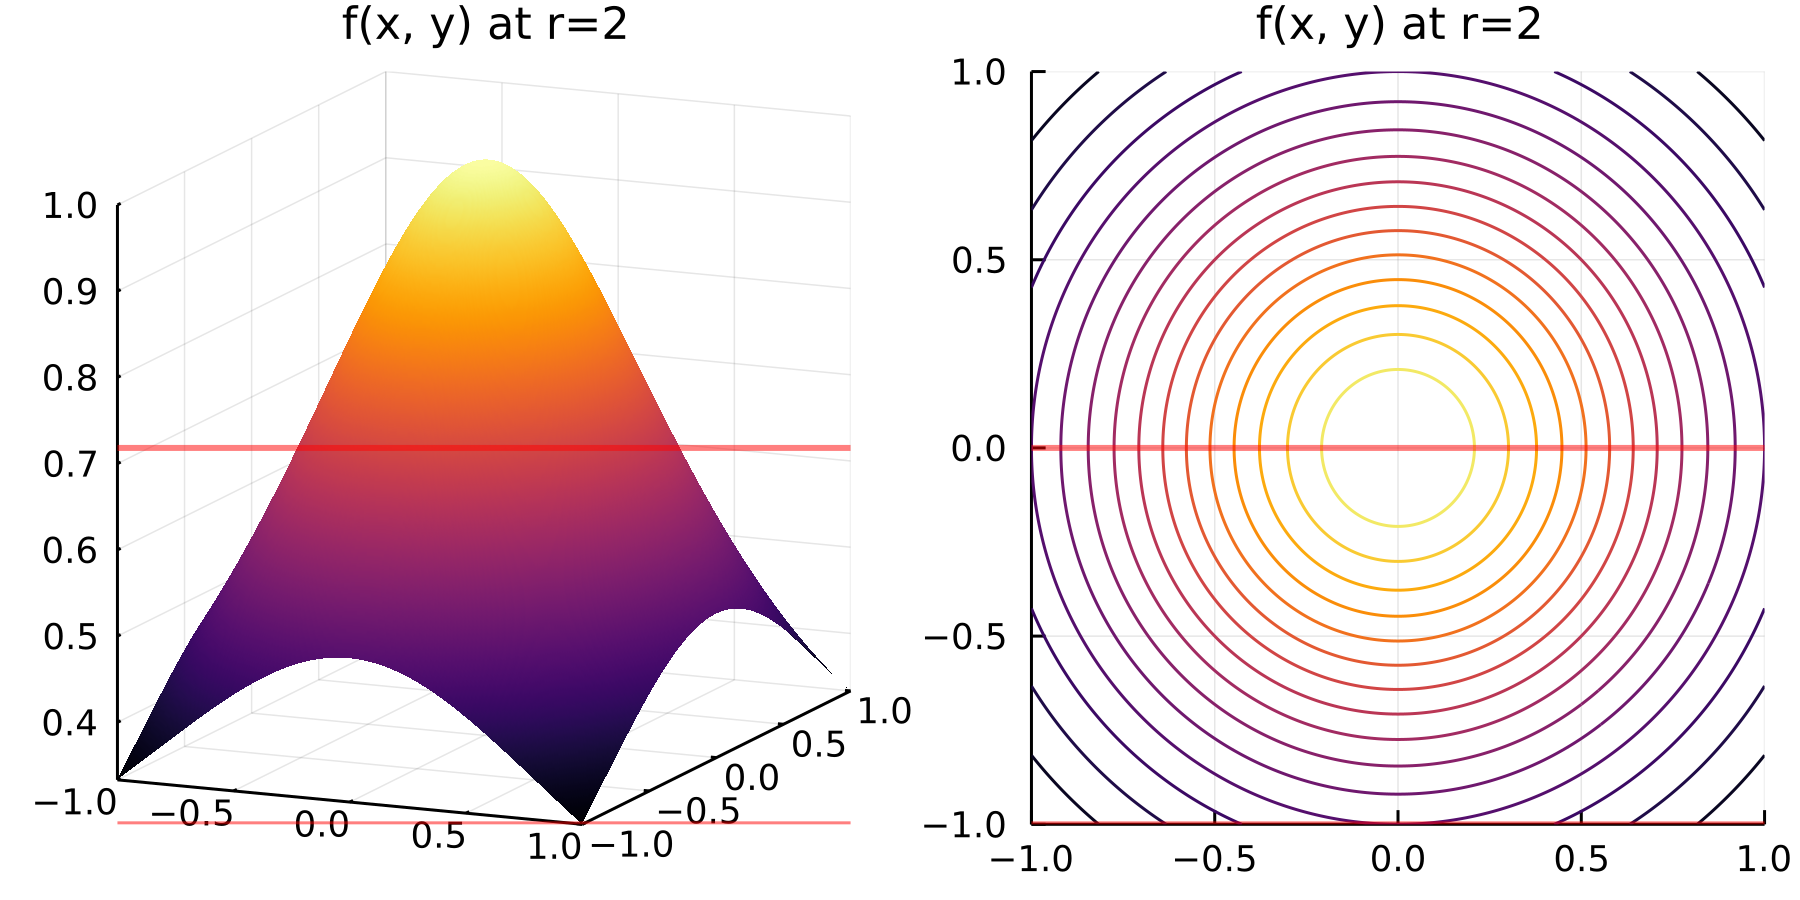
\includegraphics[width=.33\textwidth]{plots/rc-a-2.png}\hfill
    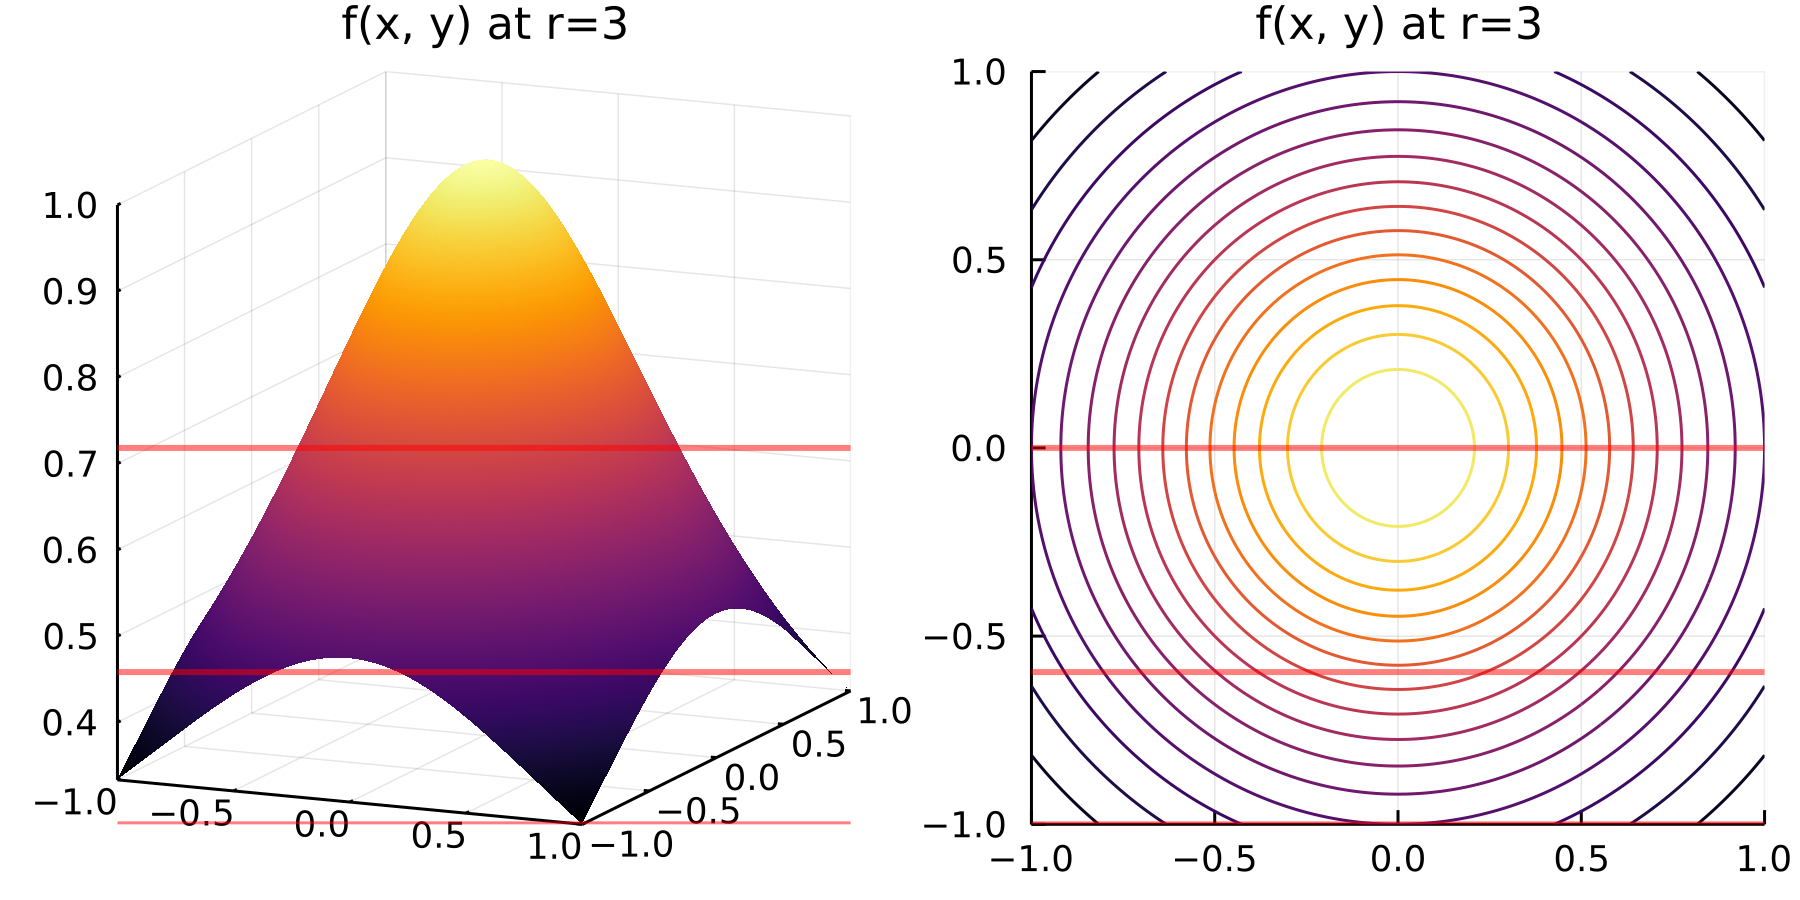
\includegraphics[width=.33\textwidth]{plots/rc-a-3.png}
    \\[\smallskipamount]
    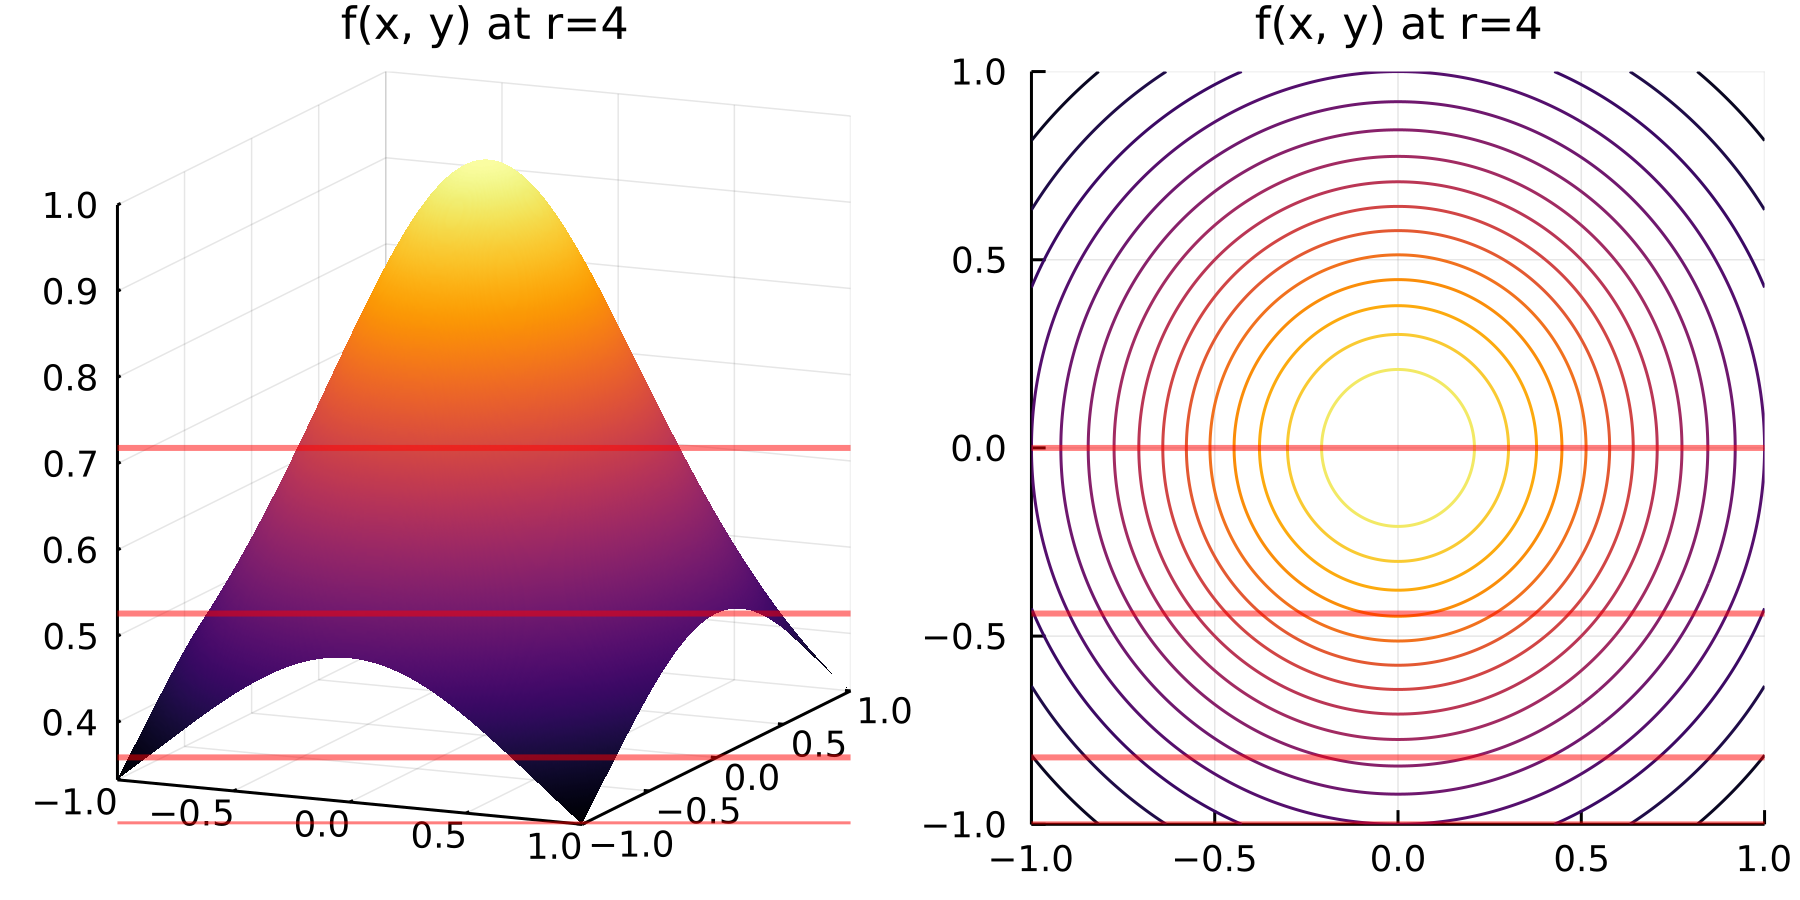
\includegraphics[width=.49\textwidth]{plots/rc-a-4.png}\hfill
    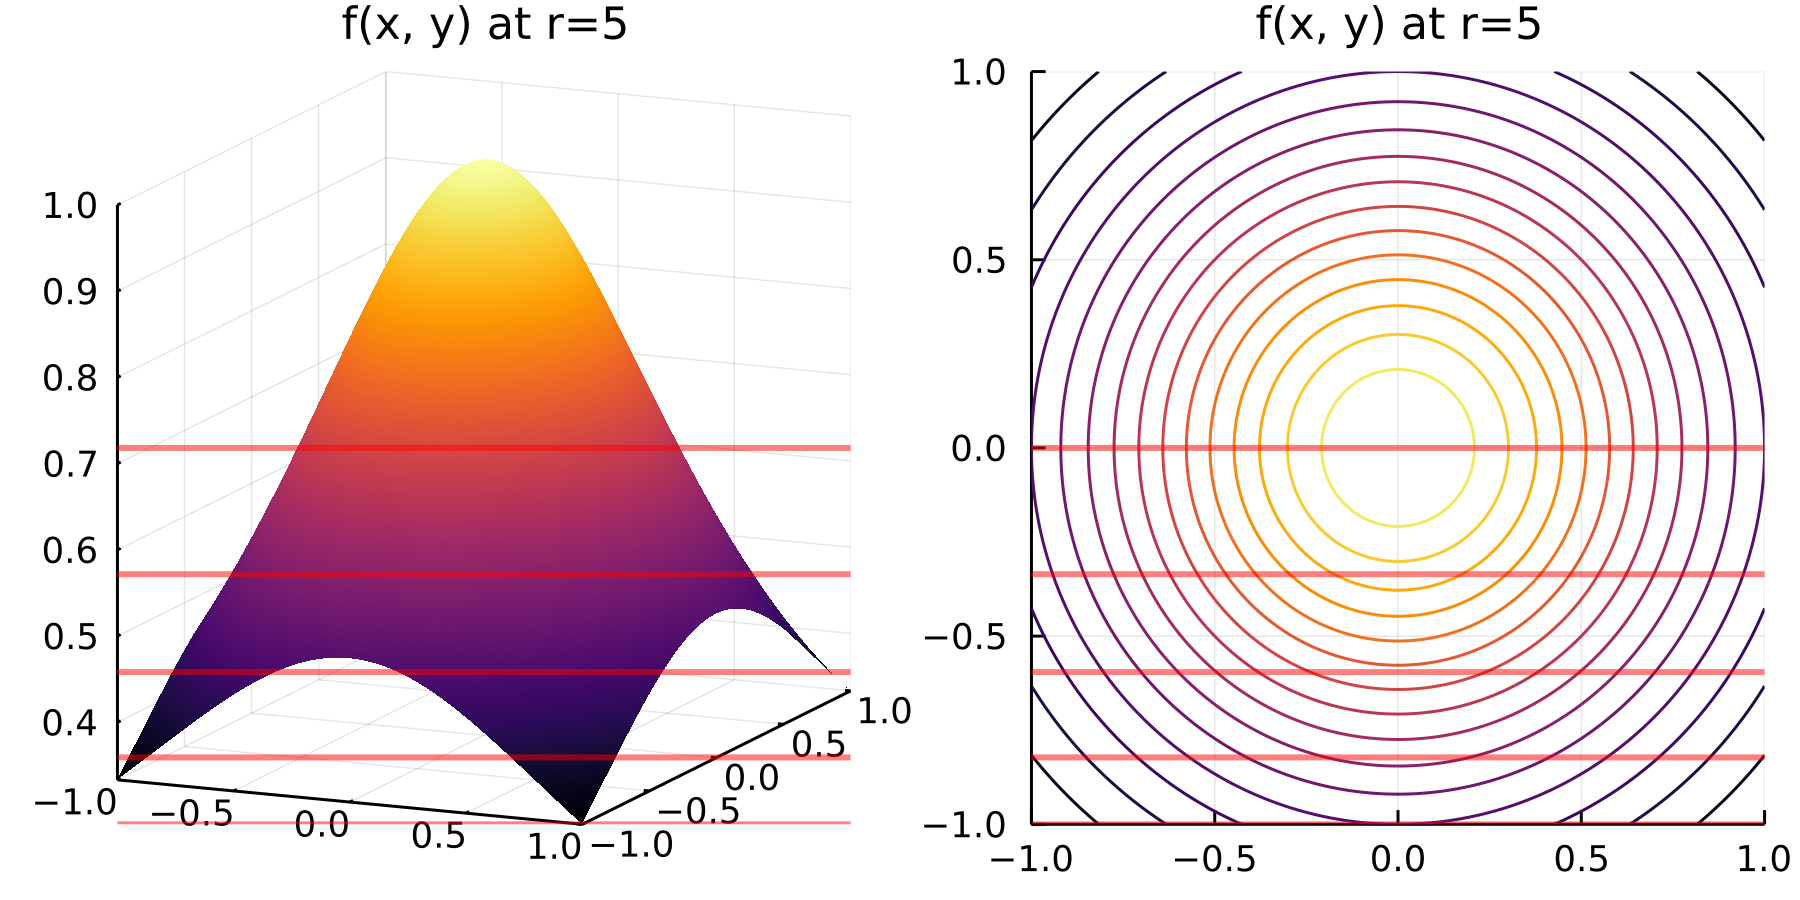
\includegraphics[width=.49\textwidth]{plots/rc-a-5.png}
    \caption{Axis-parallel lines selected by the pivoted LU, of $f(x, y)$}\label{fig:foobar}
\end{figure}
\begin{figure}[H]
    \centering
    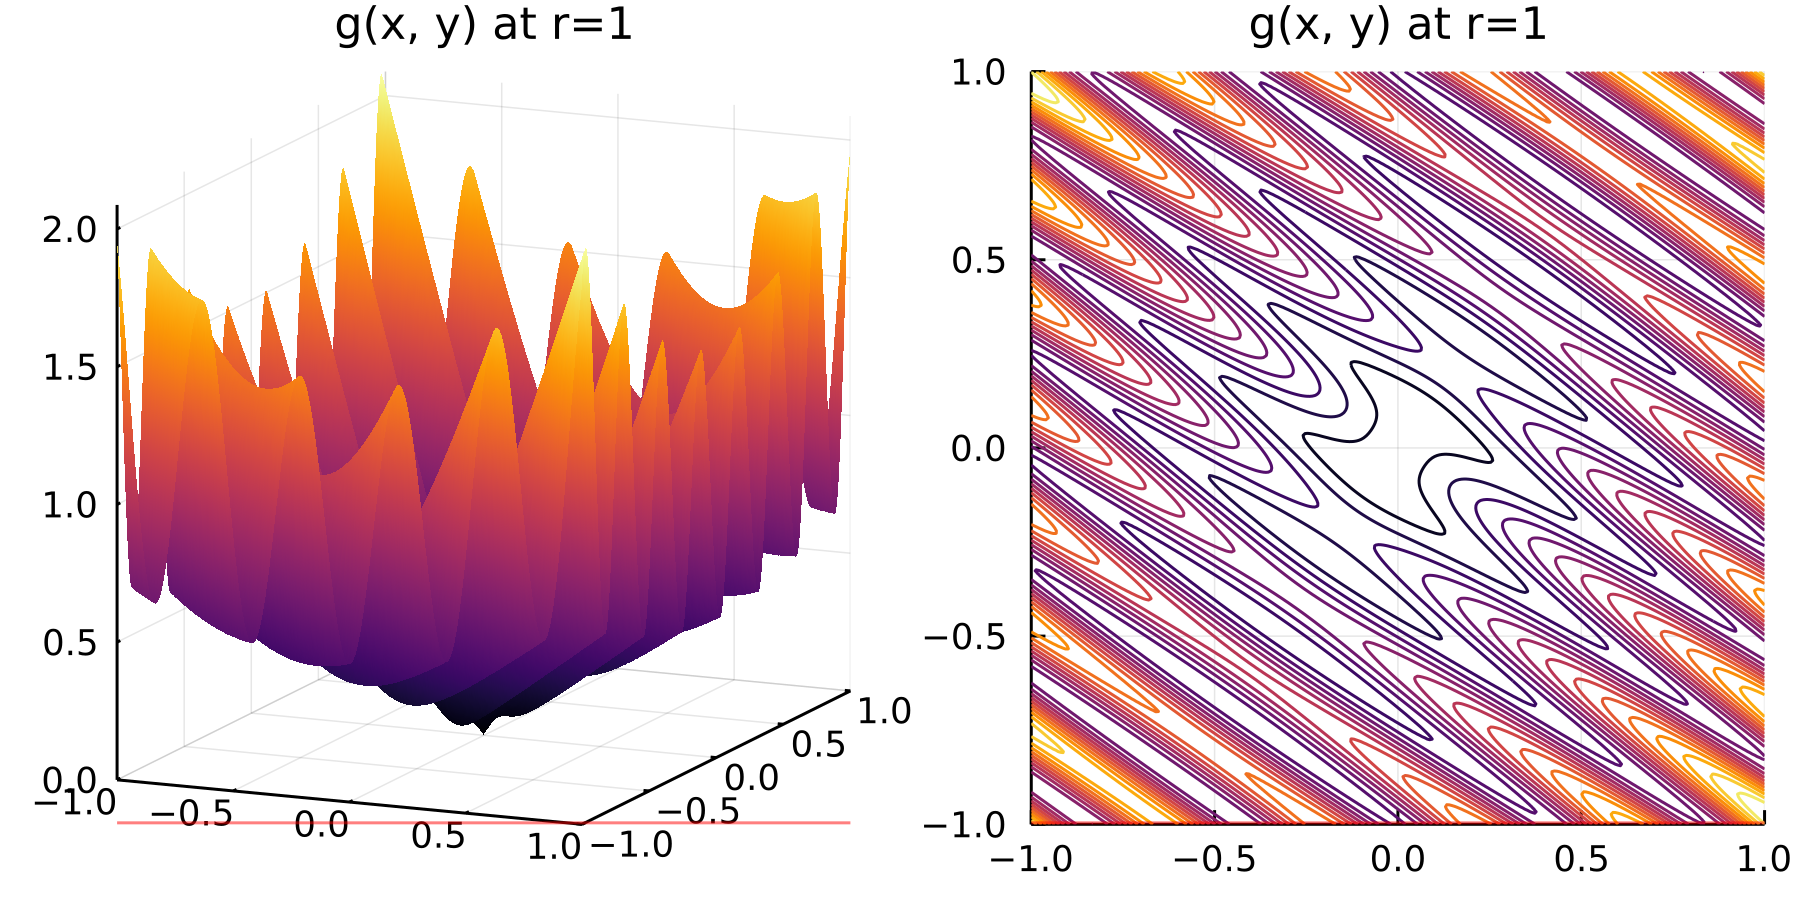
\includegraphics[width=.24\textwidth]{plots/rc-b-1.png}\hfill
    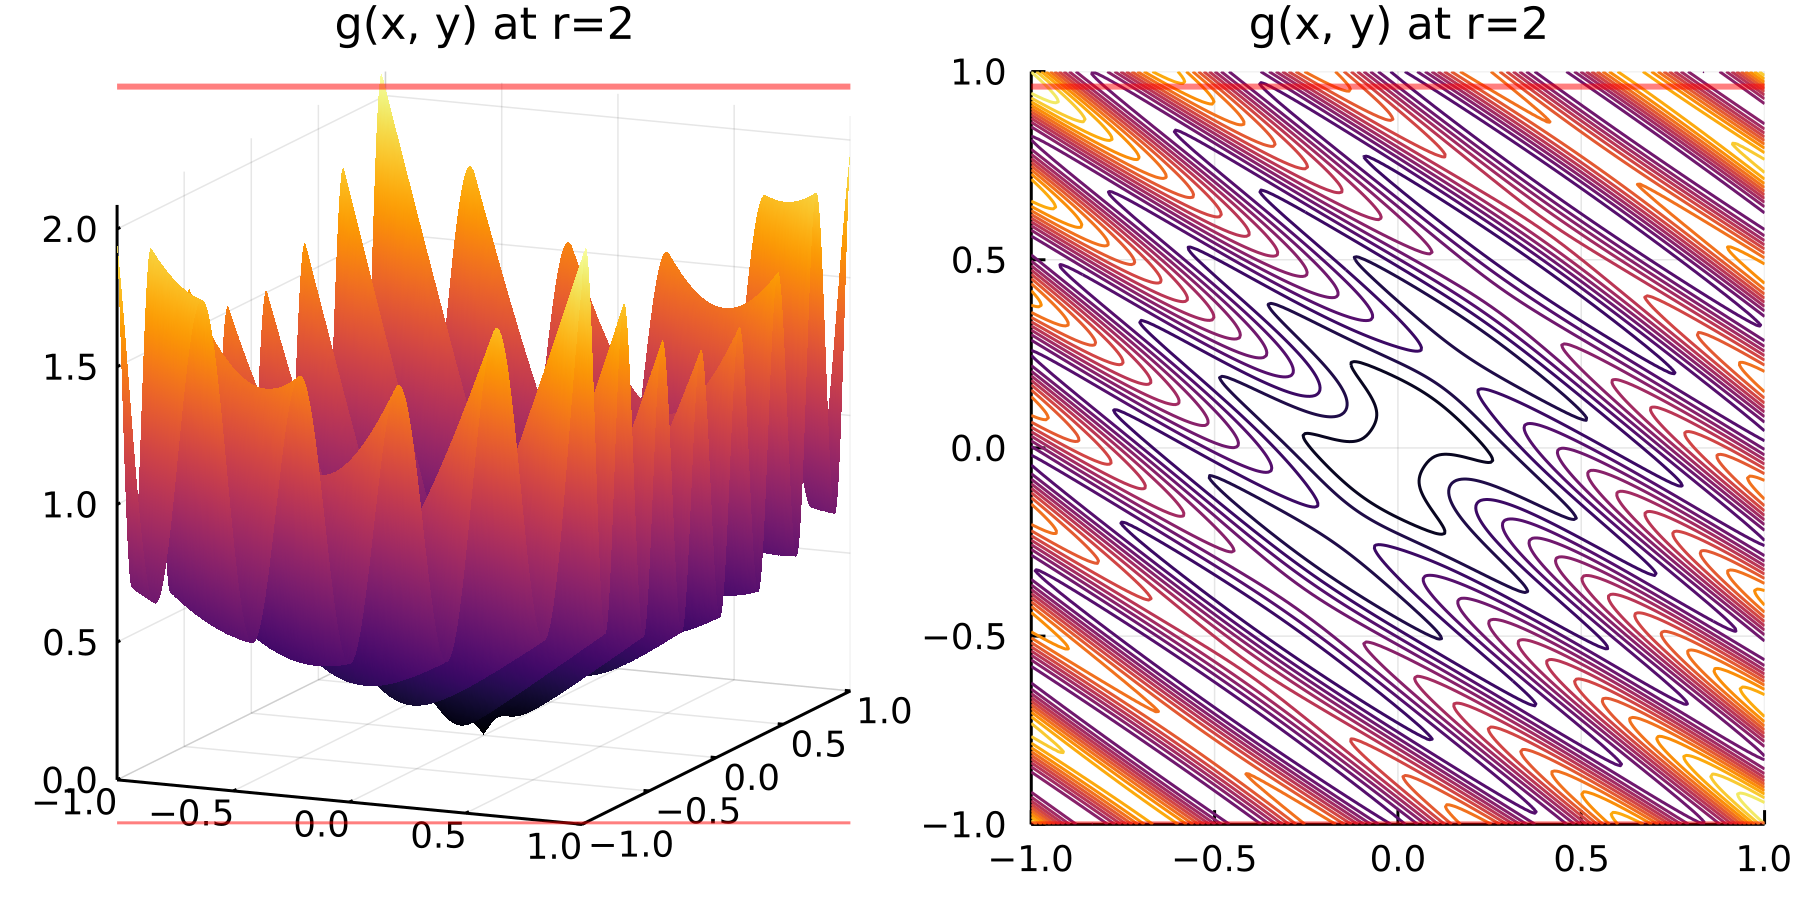
\includegraphics[width=.24\textwidth]{plots/rc-b-2.png}\hfill
    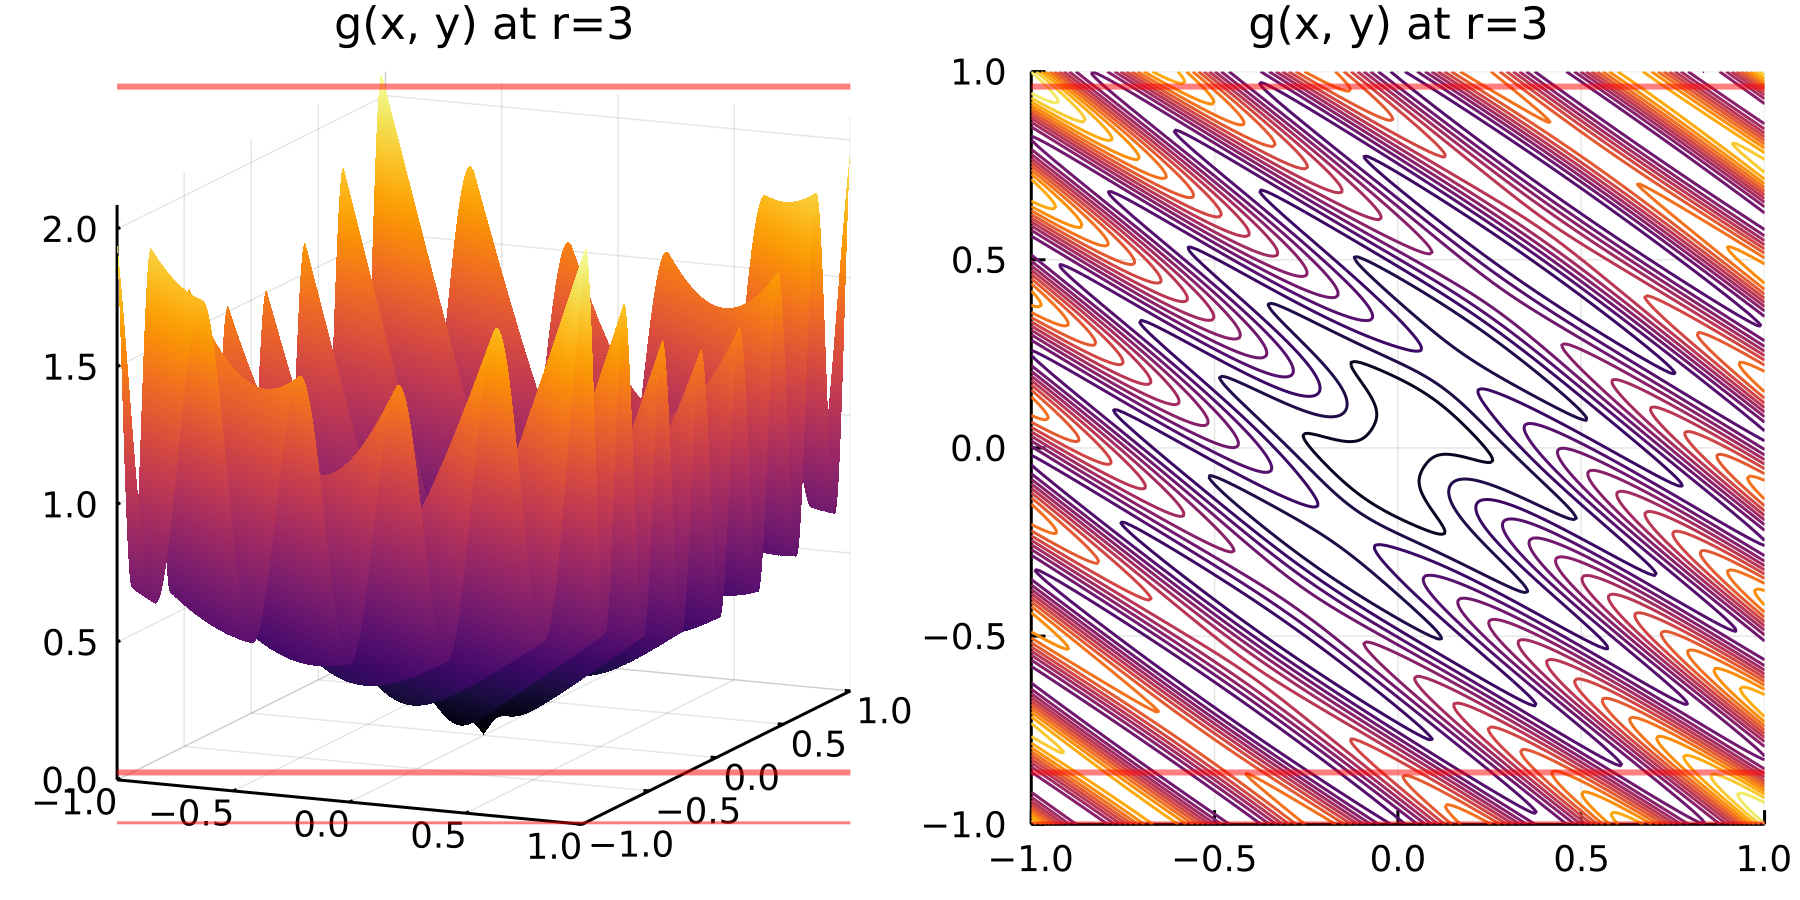
\includegraphics[width=.24\textwidth]{plots/rc-b-3.png}\hfill
    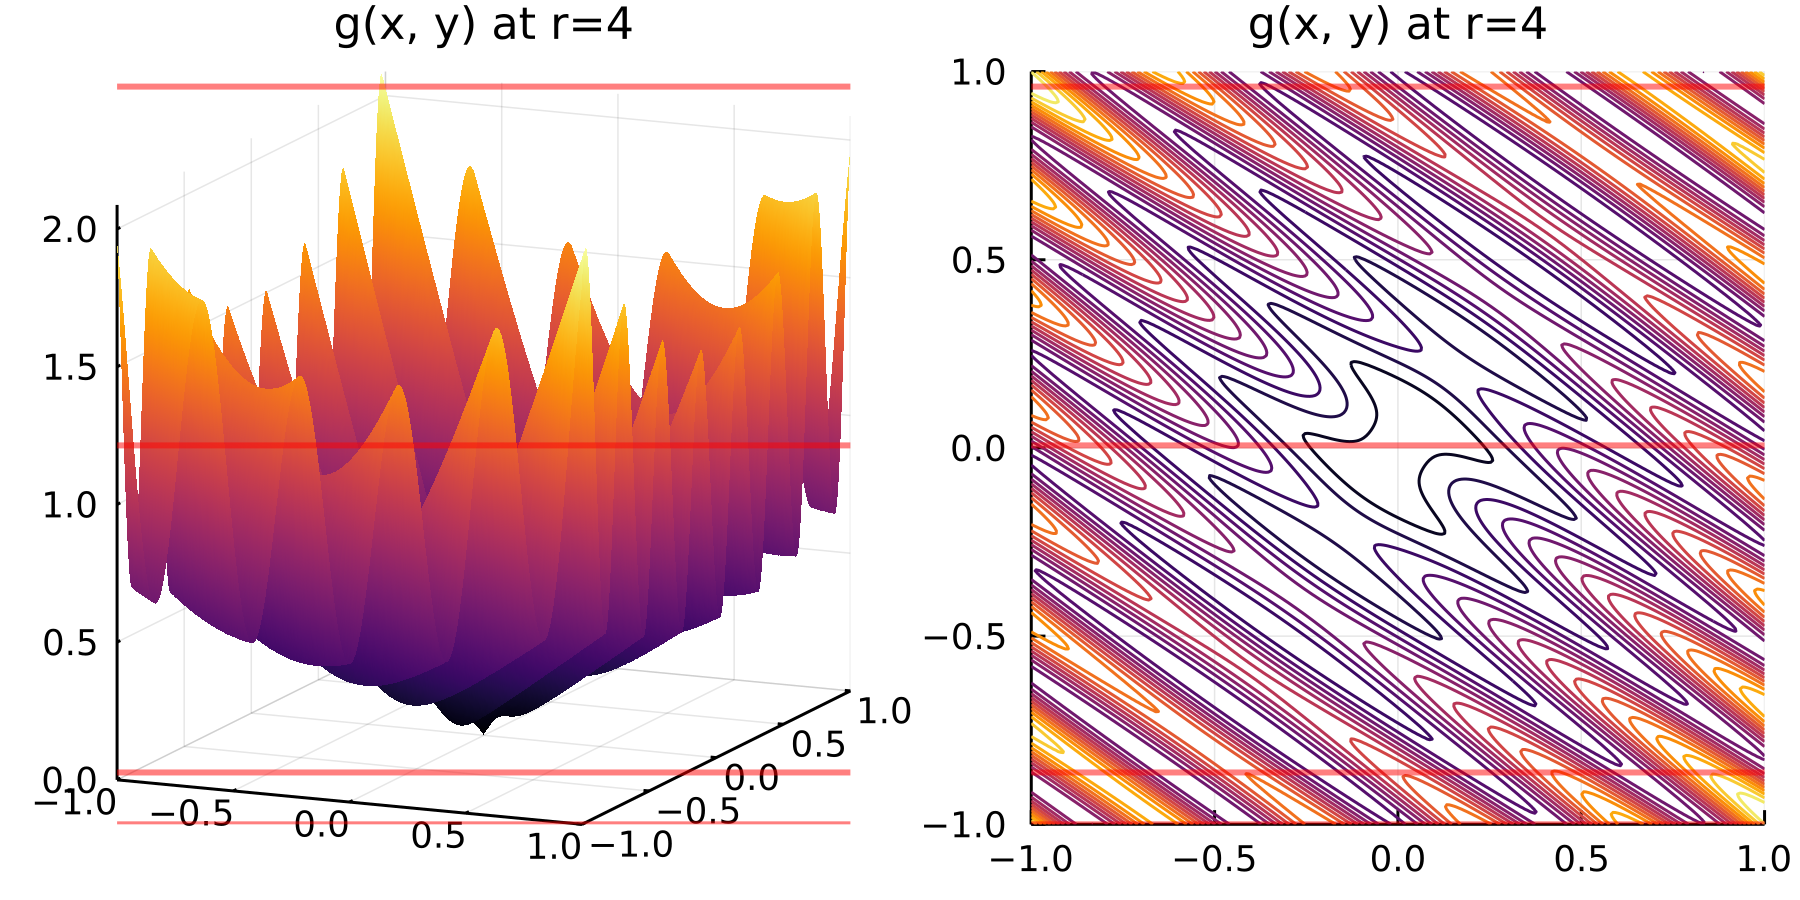
\includegraphics[width=.24\textwidth]{plots/rc-b-4.png}
    \\[\smallskipamount]
    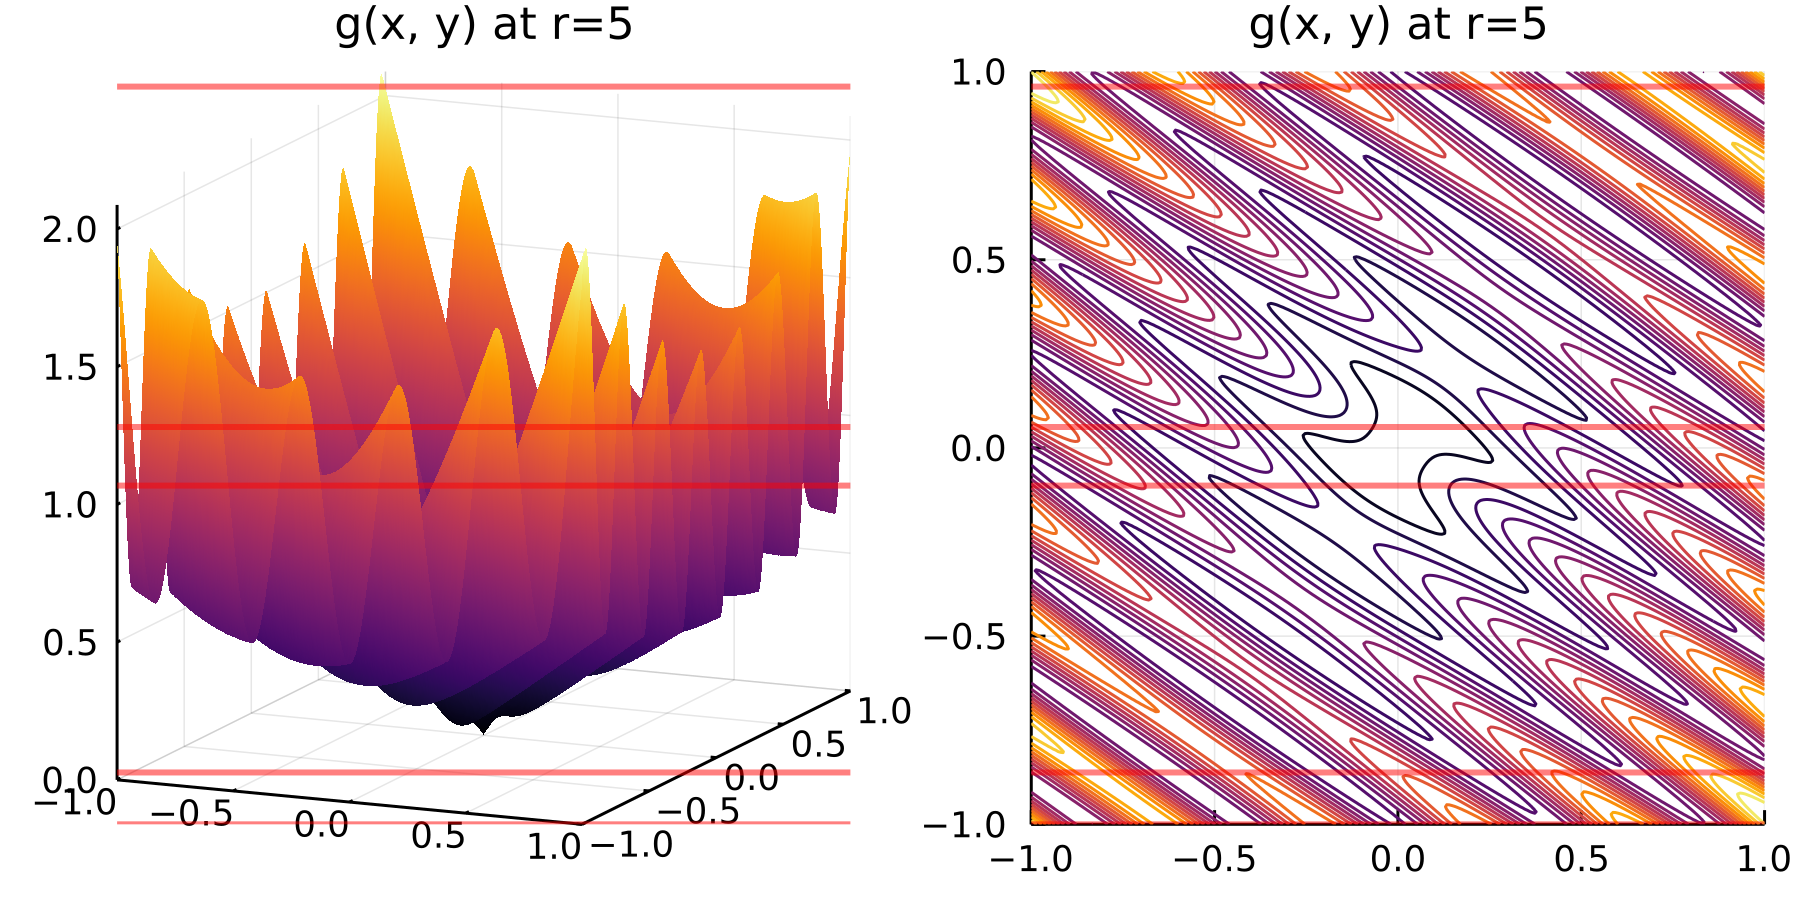
\includegraphics[width=.24\textwidth]{plots/rc-b-5.png}\hfill
    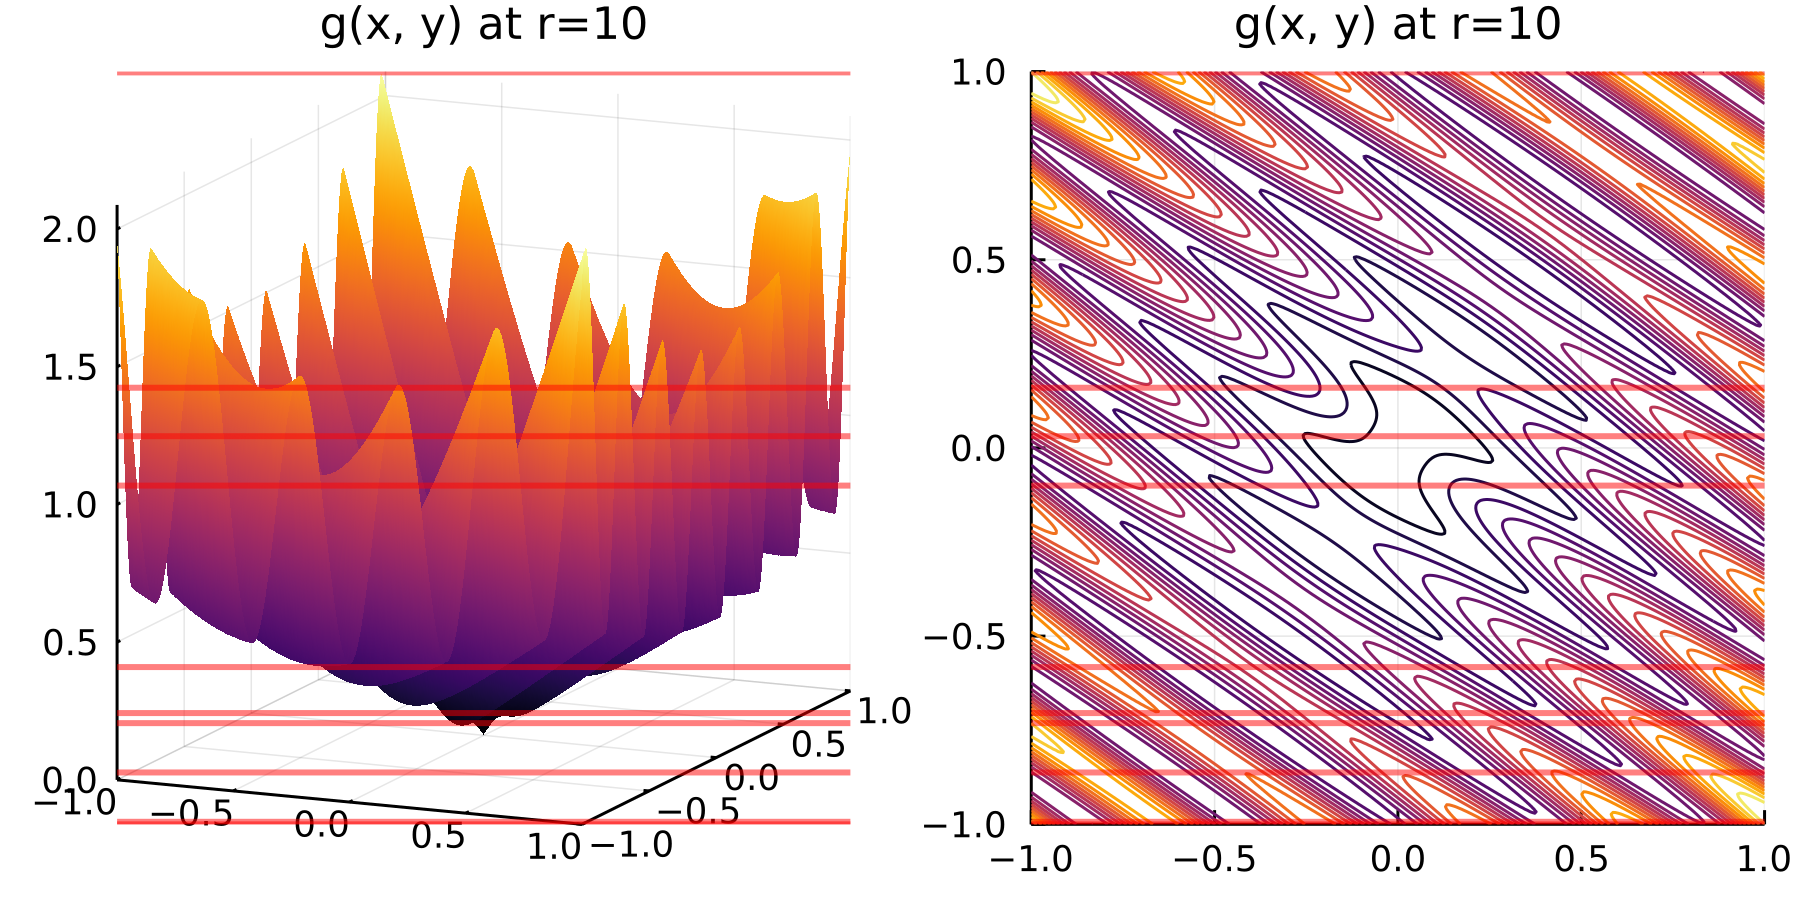
\includegraphics[width=.24\textwidth]{plots/rc-b-10.png}\hfill
    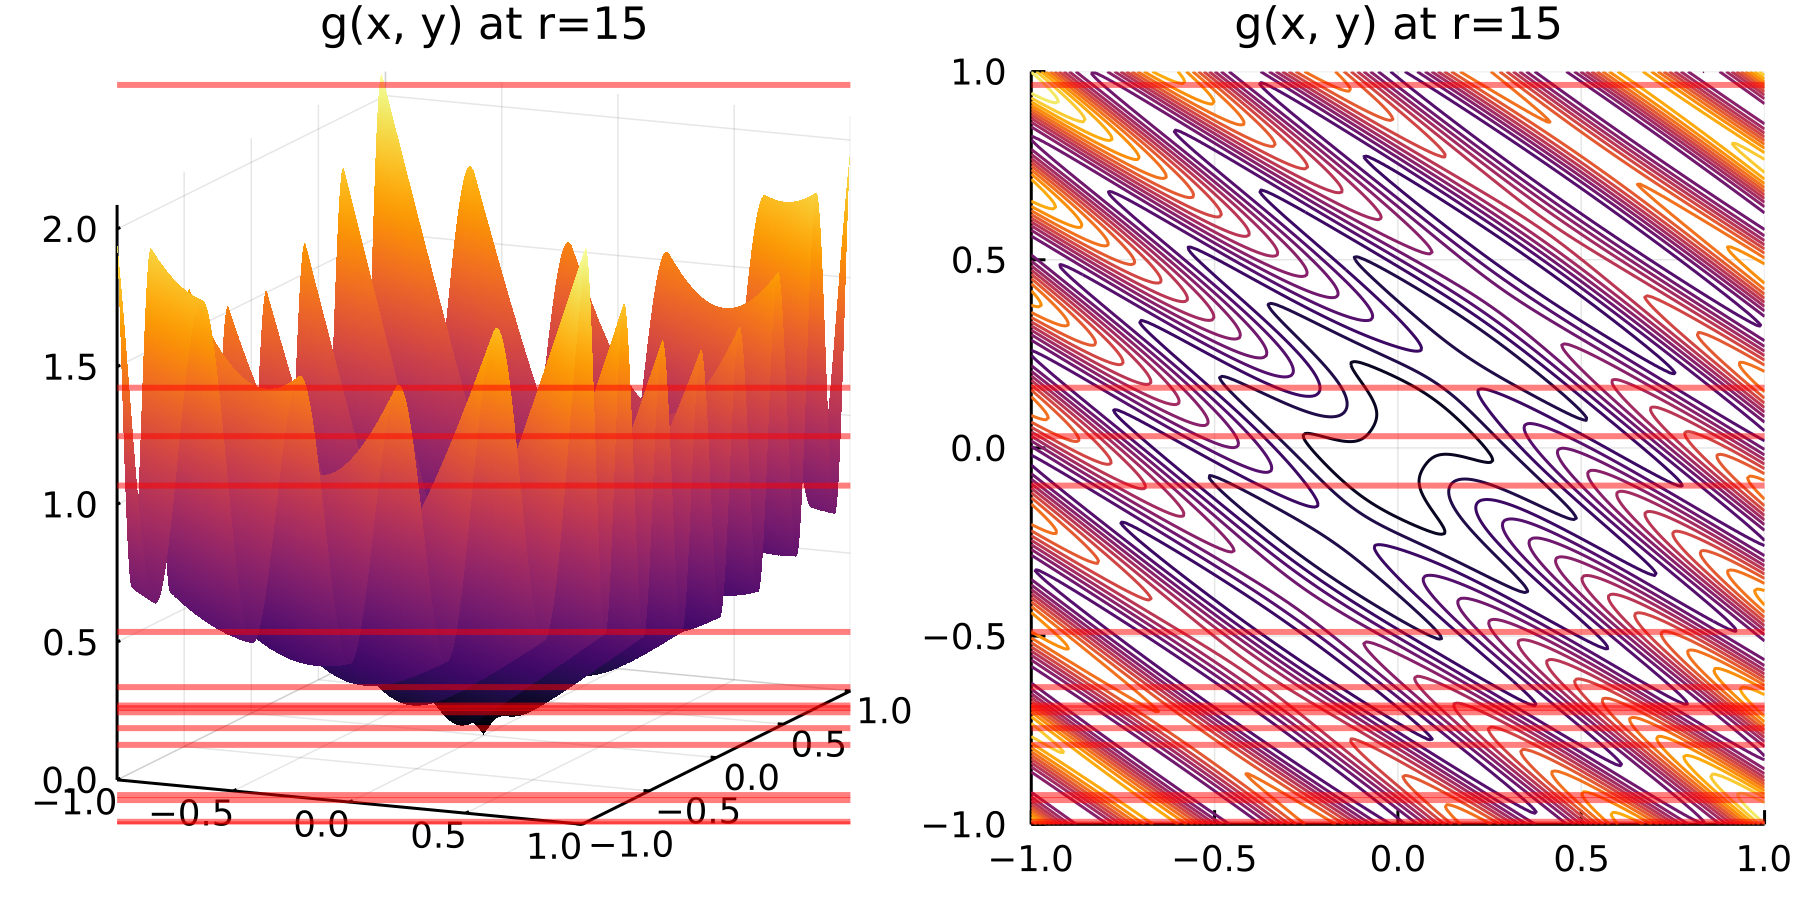
\includegraphics[width=.24\textwidth]{plots/rc-b-15.png}\hfill
    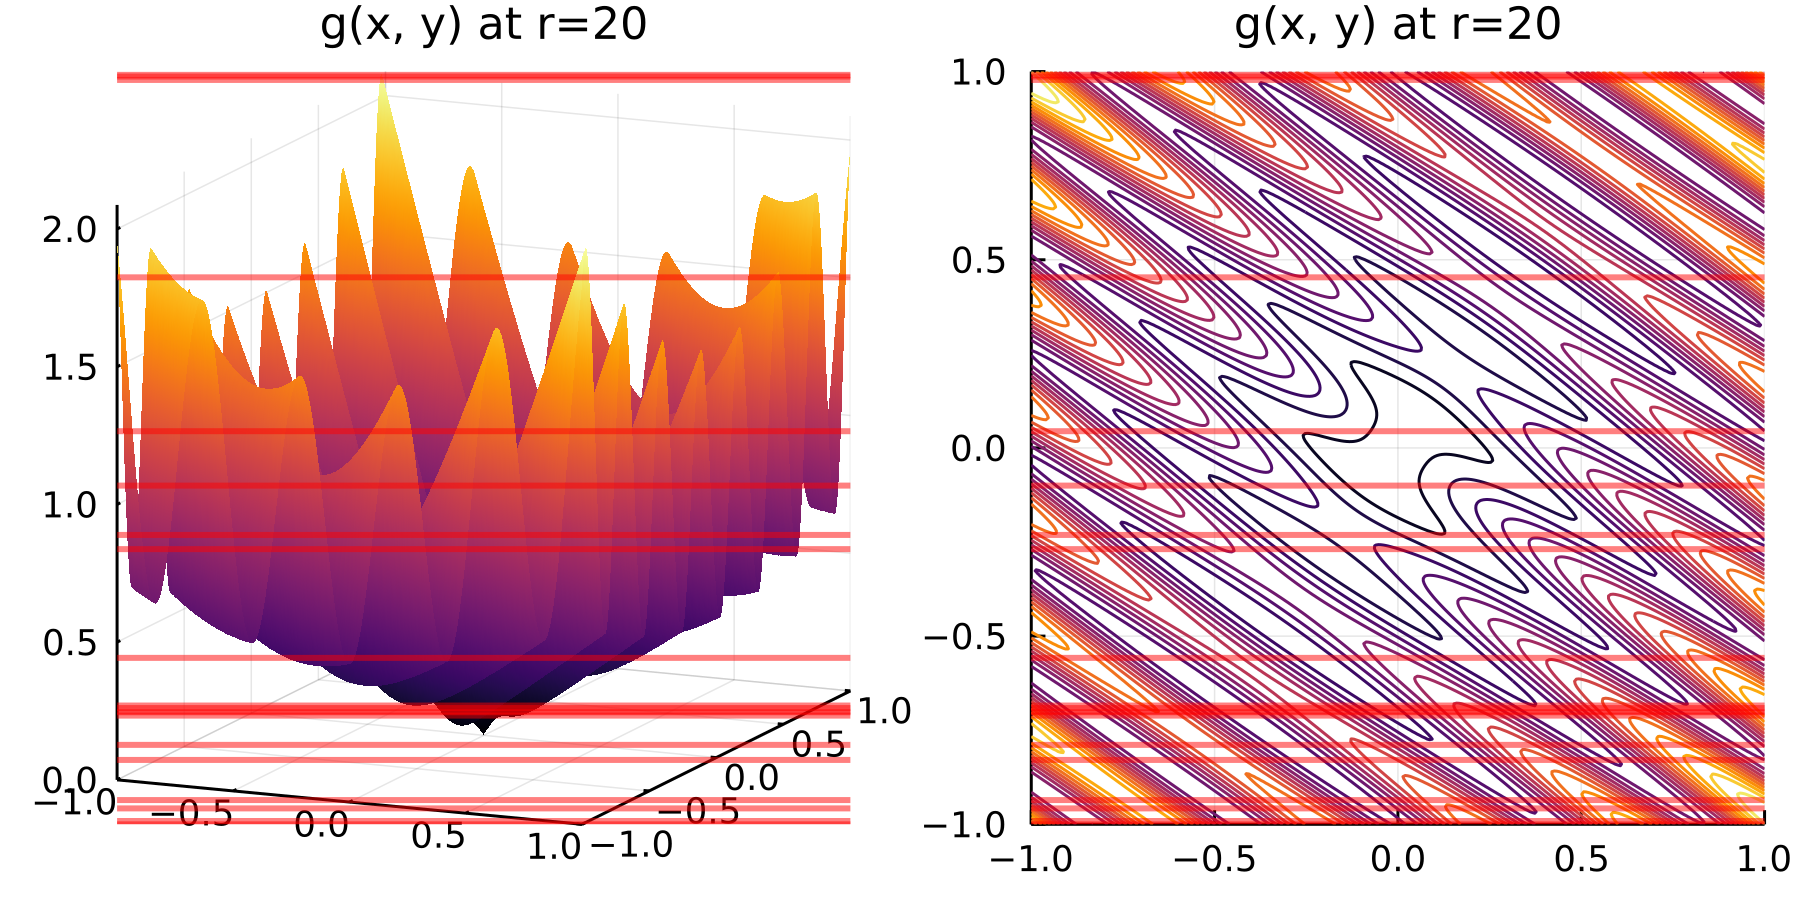
\includegraphics[width=.24\textwidth]{plots/rc-b-20.png}
    \\[\smallskipamount]
    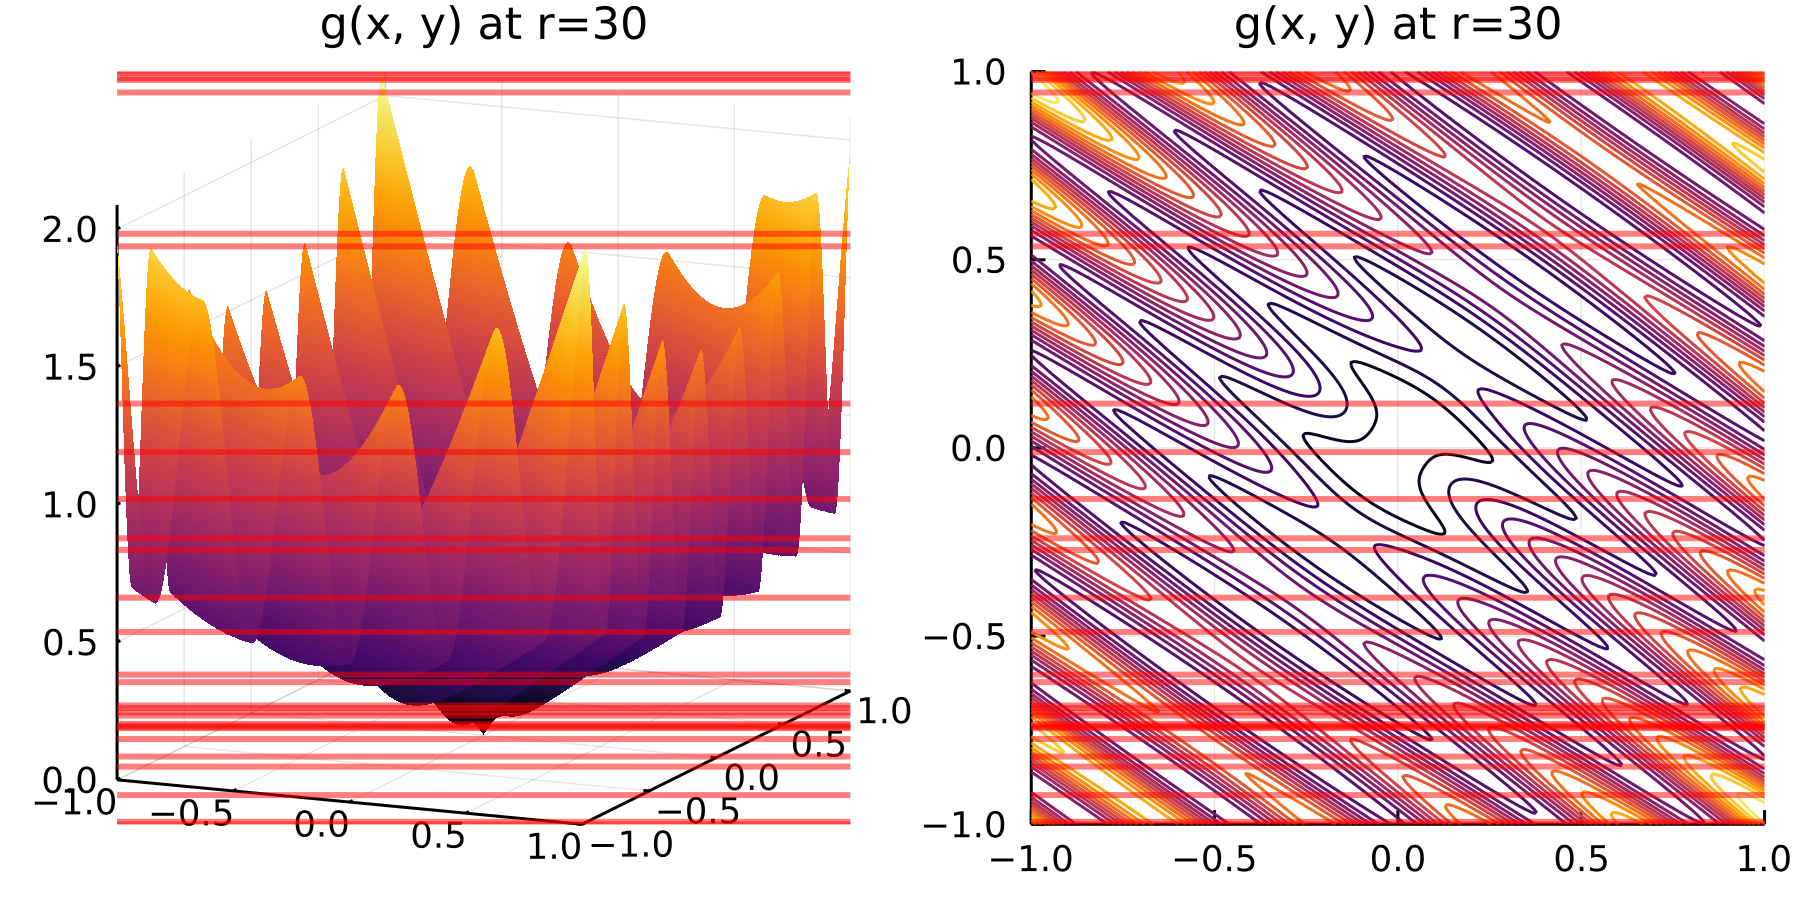
\includegraphics[width=.49\textwidth]{plots/rc-b-30.png}\hfill
    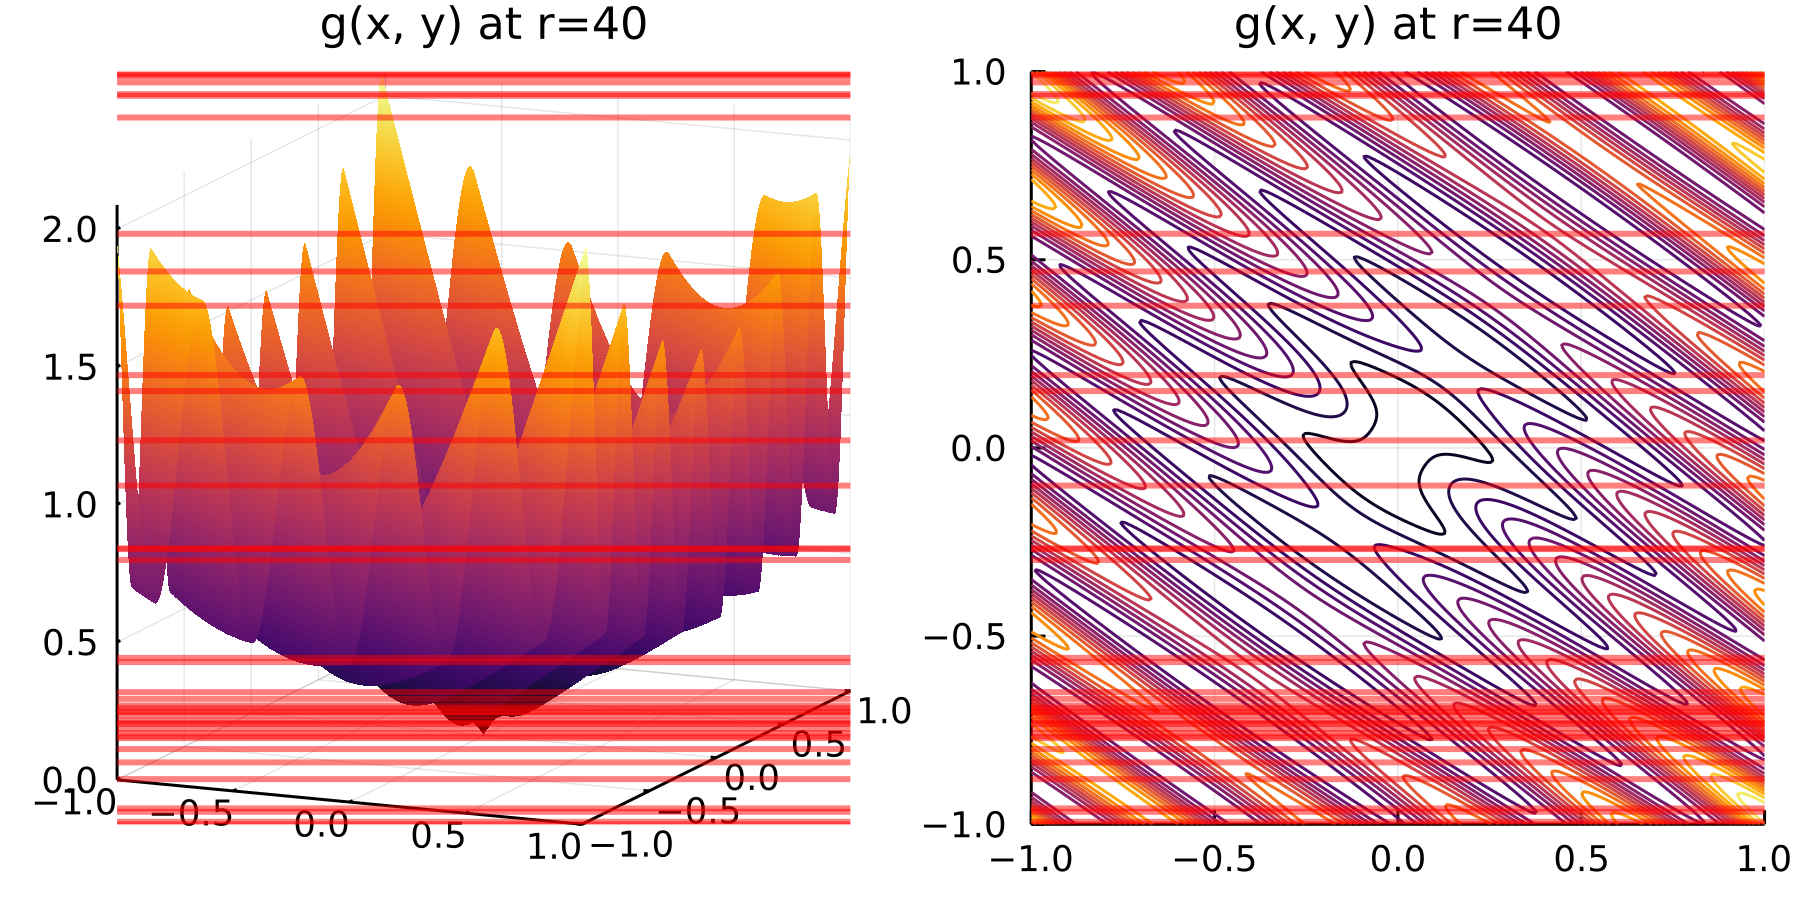
\includegraphics[width=.49\textwidth]{plots/rc-b-40.png}
    \caption{Axis-parallel lines selected by the pivoted LU, of $g(x, y)$}\label{fig:foobar}
\end{figure}

\nocite{code}
\printbibliography
\end{document}
